\documentclass[11pt]{article}
\usepackage[margin=1in]{geometry}
\usepackage{graphicx}
\usepackage{booktabs}
\usepackage{amsmath}
\usepackage{xcolor}
\usepackage{hyperref}
\usepackage{tikz}
\usetikzlibrary{positioning,arrows.meta,fit,backgrounds,calc,decorations.pathreplacing}
\hypersetup{colorlinks=true, linkcolor=blue, citecolor=blue, urlcolor=blue}

\definecolor{tgreen}{HTML}{2F6F4F}
\definecolor{tred}{HTML}{B0413E}
\definecolor{tgray}{HTML}{EEF1F0}
\definecolor{tblue}{HTML}{2B5D8A}
\definecolor{tbox}{HTML}{FFF6E0}

\newcommand{\callout}[1]{\par\vspace{2mm}\noindent\fcolorbox{black!30}{tbox}{%
\begin{minipage}{0.97\linewidth}\small #1\end{minipage}}\vspace{2mm}\par}

\title{\textbf{TOAP: The Token-Optimized Agent Protocol}\\[2mm]
\textbf{\large Reference, Summary, or KV Cache? Measuring How}\\
\textbf{\large Multi-Agent Systems Should Share Context}}
\author{Trilochan Sharma \\ Independent Researcher \\ \texttt{parnishklpo@gmail.com}}
\date{June 2026}

\begin{document}
\sloppy
\maketitle

\begin{center}\small
Code and data: \url{https://github.com/parnish007/TOAP} \quad|\quad
Code: MIT \quad|\quad Paper: CC\,BY\,4.0
\end{center}

\begin{abstract}
Multi-agent LLM pipelines tend to forward a growing transcript, the source document plus every prior
agent's output, into each downstream prompt; token cost then grows with pipeline depth. An obvious
remedy is to pass a \emph{reference} to shared content rather than re-send it. This paper measures that
remedy honestly instead of advocating for it, and the results are more nuanced than the pitch.
In a controlled experiment ($n{=}33$ real Claude generations across Haiku, Sonnet, and Opus, three
context strategies, accuracy scored by a deterministic and model-independent rubric checker),
reference-minimization (TOAP) and a competent summarizing orchestrator \emph{both} cut downstream tokens
with no accuracy loss: all 33 samples scored 4/4. But the summarizing baseline saves \emph{more} tokens
than TOAP ($\sim$2.5$\times$ vs.\ $\sim$1.9$\times$ over the naive baseline). So reference-minimization is
not a token win over good prompt engineering. What it offers instead is losslessness (a reference can be
re-expanded; a summary cannot) and security (provenance travels with the reference), and we now
\emph{measure} both rather than assert them. On a pre-registered task where a faithful summary
necessarily drops detail, a downstream responder scores \textbf{8/8 with the reference vs.\ 6/8 with the
summary}, failing exactly on the dropped facts. Against an adversarial corpus of 40 attacks across
nine categories, the capability lattice blocks \textbf{all 40} attempts to drive a side-effecting
operation from untrusted content with \textbf{zero} false positives on 14 benign read/analysis
requests. That guarantee does not depend on how an injection is phrased, and we show its two documented
blind spots as well. (An accuracy regression we first saw on Haiku at $n{=}1$ did not reproduce at
$n{=}5$ and is retracted, a small lesson in why single-call agent measurements are unsafe.) On the
compute side, we implement and measure the third materialization, a same-model KV-cache transfer,
across seven open models: reusing a transferred prefix cache is a real, near-lossless prefill speedup
(35/36 cells byte-identical; up to $\sim$180$\times$ at long context), but the cache is thousands of
times larger than the text, so it only pays off when agents are co-located or use grouped-query
attention. That last result grounds TOAP's gating policy in measurement rather than assumption.
Throughout we separate wire bytes from model tokens, and show symbolic ``opcodes'' save 50\% of bytes
but only 0--17\% of tokens. We describe the protocol architecture (a two-plane wire format; a
reference-materialization spectrum) and a Rust reference implementation. \emph{Threats to validity are
first-class}: a single model family/tokenizer for the token study, a same-family judge as a secondary
check only, and small $n$. The mechanism is not novel (blackboard systems, A2A artifacts, ADOL); the
contribution is the honest, reproducible accounting.
\end{abstract}

\section{Introduction}
In agent pipelines and fan-out workflows, an orchestrator typically forwards a growing transcript into
each subsequent agent's prompt. Because LLM cost is paid per prompt token, redundant re-transmission
dominates coordination cost. TOAP stores shared content once under an identifier and exchanges
references, so each agent retrieves only what it needs.

We try to be conservative about what this buys. The underlying mechanism is old (\S\ref{sec:related}),
and ``$10\times$'' claims that count bytes rather than tokens are misleading (\S\ref{sec:bytes}). The
question worth asking is not whether referencing saves tokens, but how it compares to a competently
engineered baseline. Our first result is a little humbling: on an easy task a good summarizing
orchestrator saves \emph{more} tokens than reference-minimization at the same accuracy. We treat this
as the start of the argument, not the end of it.

\emph{Thesis.} No single way of sharing context dominates. A summary is cheapest in tokens but lossy;
a reference is lossless and carries security metadata but costs more tokens; a transferred KV cache is
the fastest to consume but is enormous and model-bound. Which one wins depends on the regime --- the
length of the shared context, the model's attention architecture, whether producer and consumer are
co-located, and whether a later step might need a detail an upfront summary would discard. The
contribution of this paper is to \emph{measure} those regime boundaries rather than assume them, and to
give an architecture (TOAP) whose reference primitive can be \emph{materialized} as inline text, a
context id, or a KV pointer accordingly. Each of the three following claims is now backed by a
measurement: the summary's lossiness costs downstream accuracy on a task that needs a dropped detail
(\S\ref{sec:lossless}); the capability lattice blocks a corpus of injection attempts with no false
positives (\S\ref{sec:security-eval}); and KV transfer's compute win, and its size cost, are mapped
across seven models (\S\ref{sec:kv-results}).

\callout{\textbf{What is measured vs.\ proposed.} The token experiments (\S\ref{sec:bytes},
\S\ref{sec:results}) use the implemented V1 text protocol and real model generations; the KV-bridge
experiment (\S\ref{sec:kv-results}) uses the implemented same-model prefix-reuse sidecar.
\textbf{\S\ref{sec:arch:status} states precisely what is implemented today} (V1/V2 protocol, the
context store with capability-lattice security, the materialization policy, and the KV-bridge sidecar)
\textbf{and what remains future work} (durable/distributed store, cross-vendor evaluation, message
signing).}

\noindent\textbf{Contributions.}
\begin{enumerate}\itemsep1pt
  \item A two-plane protocol architecture and a reference-materialization spectrum (\S\ref{sec:arch}),
        with a Rust reference implementation (\S\ref{sec:impl}).
  \item An honest token accounting separating bytes, tokens, and compute, including the result that a
        summarizing baseline beats referencing on tokens (\S\ref{sec:bytes}, \S\ref{sec:results}).
  \item A pre-registered demonstration that a summary's lossiness costs downstream accuracy when a
        dropped fact is needed, while a reference does not (\S\ref{sec:lossless}).
  \item An adversarial evaluation of the capability lattice against a corpus of injection attempts
        (\S\ref{sec:security-eval}).
  \item A seven-model measurement of same-model KV-cache reuse, mapping where its compute win justifies
        the cache-transfer cost (\S\ref{sec:kv-results}).
\end{enumerate}

\section{Background and Related Work}\label{sec:related}
\textbf{Shared-store coordination.} Agents coordinating through a common store rather than passing full
messages is the \emph{blackboard} model (Hearsay-II~\cite{erman1980}); database normalization and
pointers are the same principle. TOAP's context store is a modern restatement, and we claim no novelty
for it. \textbf{Agent protocols.} MCP~\cite{mcp} (agent--tool) and A2A~\cite{a2a} (agent--agent) are
the dominant standards; A2A already references shared content by ID via \emph{artifacts}. Token bloat
is recognized: the ADOL Internet-Draft~\cite{adol} and MCP SEP-1576 target token-efficient messaging
(Table~\ref{tab:landscape}). \textbf{Caching.} Provider prompt caching~\cite{promptcache} realizes
``send once, reference implicitly'' within one provider/session; cross-agent referencing is
complementary. \textbf{Symbolic comms}~\cite{talkhier,codeagents} cut tokens but risk comprehension;
we measure the opcode component at $\le$17\%. \textbf{Security.} Provenance tracking follows CaMeL~\cite{camel}.
\textbf{KV reuse}~\cite{kvcomm} is crowded and is treated as an optional, constraint-guarded mode.

\begin{table}[h]\centering\footnotesize
\begin{tabular}{llll}
\toprule
Protocol & Layer & Wire format & Token efficiency a goal? \\
\midrule
MCP (Anthropic) & agent--tool & JSON-RPC 2.0 / HTTP & No \\
A2A (Google/LF) & agent--agent & JSON-RPC/HTTP (+gRPC/REST) & No \\
ADOL (IETF draft) & layer above MCP/A2A & JSON \texttt{\$ref} dedup & Yes (content selection) \\
\textbf{TOAP (this work)} & agent--agent & two-plane text/binary & Yes (encoding, token-aware) \\
\bottomrule
\end{tabular}
\caption{Inter-agent protocol landscape (2026). TOAP is adjacent to ADOL/SEP-1576, not ahead of them.}
\label{tab:landscape}
\end{table}

\section{Bytes Are Not Tokens}\label{sec:bytes}
A common mistake is to minimize \emph{bytes} and report the result as token savings. The two are not
the same. BPE tokenizers pre-tokenize on punctuation before merging, so a payload dense in punctuation
spends close to one token per symbol. Measured with \texttt{tiktoken} (cl100k),
\texttt{SUM(CTX:42)?max\_words=150} is 25 bytes and 10 tokens, while the natural-language ``Please
summarize document 42 in at most 150 words.'' is 50 bytes and 12 tokens: half the bytes, but only 17\%
fewer tokens (Figure~\ref{fig:bytes}). Richer payloads save even less. The lesson is that opcode terseness
is a minor lever, and the question that actually matters is whether to transmit the \emph{content} at
all. We keep three cost planes separate throughout this paper and measure each on its own terms: wire
bytes, model-input tokens, and prefill compute.

\begin{figure}[h]\centering
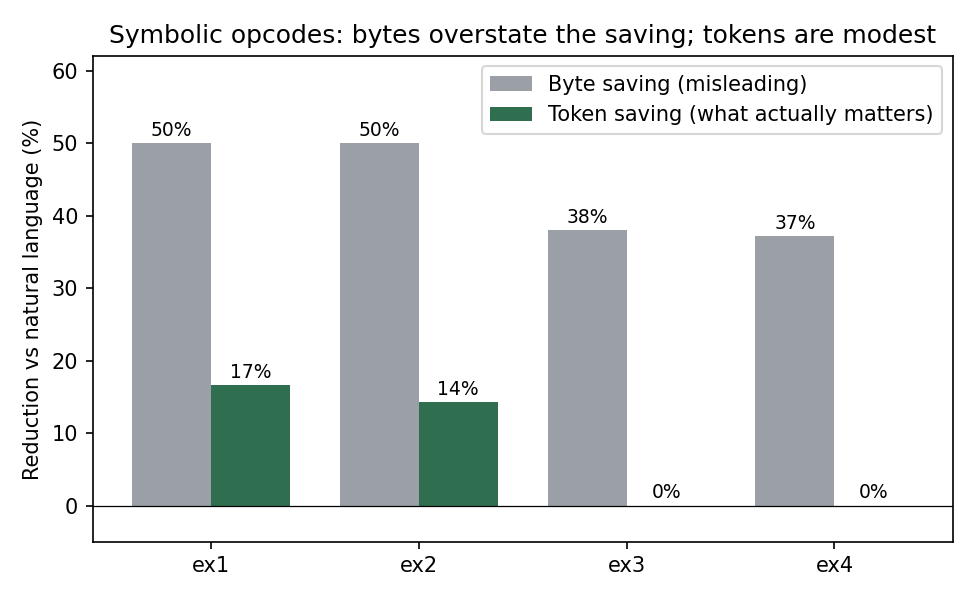
\includegraphics[width=0.62\textwidth]{figures/fig_bytes_tokens.png}
\caption{Byte savings overstate token savings for symbolic opcodes (tiktoken cl100k).}
\label{fig:bytes}
\end{figure}

\section{TOAP Architecture}\label{sec:arch}
\subsection{System overview}
TOAP is a layered, broker-mediated protocol (Figure~\ref{fig:arch}). A message travels \emph{down} the
stack on the way out and \emph{up} the stack on the way in, and each layer has one narrow job. The
choice that shapes everything else is that \textbf{agents never talk to each other directly}: every
message goes through a broker that owns identity, access control, and routing. We made that choice on
purpose. If an agent could open a socket to another agent, then the ``who sent this'' field would have
to be either trusted (spoofable) or separately authenticated on every edge of the mesh; routing the
mesh through one mediator means identity is decided once, at the point of connection, and never has to
be claimed on the wire again. It also gives security a single place to live (\S\ref{sec:arch:security})
instead of being re-implemented in every agent. The cost is a central dependency, which we treat as an
explicit assumption rather than pretend away (\S\ref{sec:disc}).

To make the layers concrete before defining them one by one, it helps to follow a single request all
the way through. Suppose an orchestrator wants a worker to summarize a document it holds. The document
is stored once; the request that crosses the wire is a short reference, not the text; the reply comes
back correlated to the original request; and at no point does the worker learn, or get to assert, who
the orchestrator is. Figure~\ref{fig:trace} traces exactly that, and the per-layer subsections below
explain what each step does and why it is built the way it is. After the layers we cover the two ideas
that are particular to TOAP: the two-plane wire format (\S\ref{sec:twoplane}) and the reference
materialization spectrum (\S\ref{sec:refspec}).

\begin{figure}[h]\centering
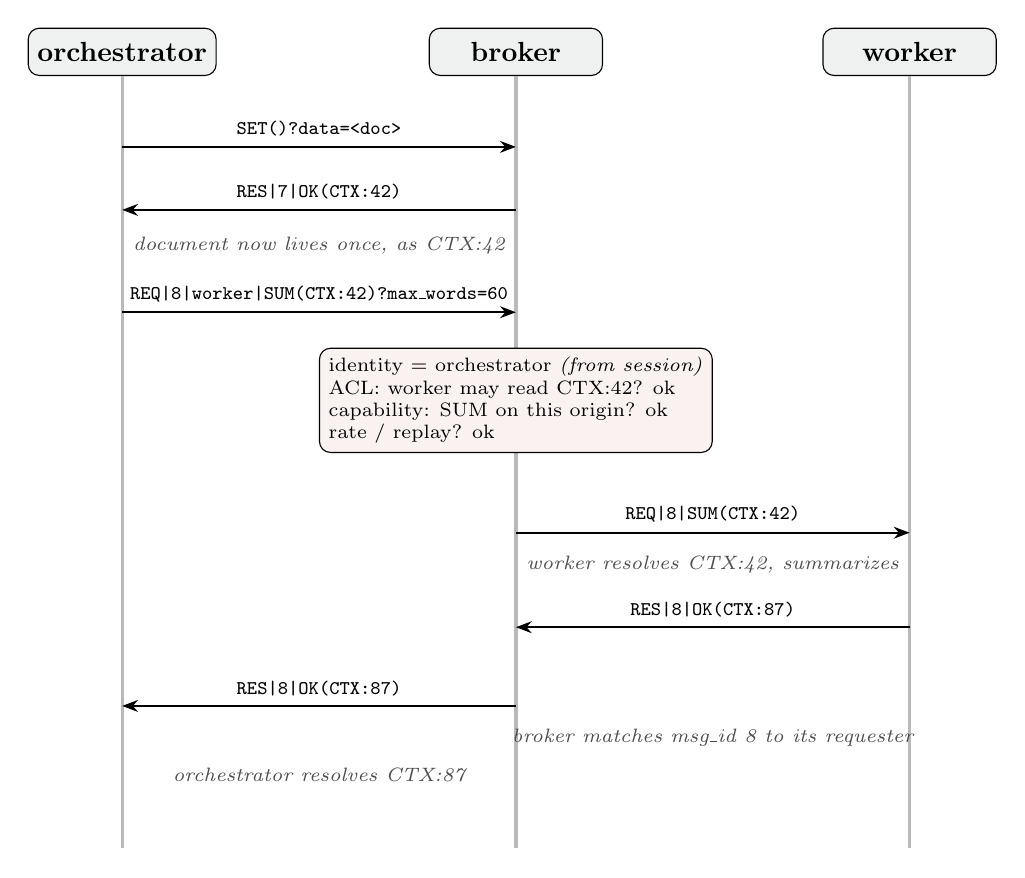
\begin{tikzpicture}[font=\footnotesize,
  lifeline/.style={very thick, gray!55},
  head/.style={draw, rounded corners, fill=tgray, minimum width=2.2cm, minimum height=0.6cm, font=\bfseries},
  msg/.style={-{Stealth[length=2mm]}, thick},
  note/.style={font=\scriptsize\itshape, gray!60!black}]
% actors
\node[head] (O) at (0,0) {orchestrator};
\node[head] (B) at (5,0) {broker};
\node[head] (W) at (10,0) {worker};
\foreach \n in {O,B,W} \draw[lifeline] (\n.south) -- ++(0,-9.8);
\def\y{-0.9}
% 1. store (orchestrator -> broker -> back)
\draw[msg] ($(O.south)+(0,\y)$) -- node[above,font=\scriptsize]{\ttfamily SET()?data=<doc>} ($(B.south)+(0,\y)$);
\draw[msg] ($(B.south)+(0,\y-0.8)$) -- node[above,font=\scriptsize]{\ttfamily RES|7|OK(CTX:42)} ($(O.south)+(0,\y-0.8)$);
\node[note] at ($(O.south)!0.5!(B.south)+(0,\y-1.25)$) {document now lives once, as CTX:42};
% 2. request (orchestrator -> broker)
\draw[msg] ($(O.south)+(0,\y-2.1)$) -- node[above,font=\scriptsize]{\ttfamily REQ|8|worker|SUM(CTX:42)?max\_words=60} ($(B.south)+(0,\y-2.1)$);
% broker self-checks (box sits on the broker lifeline, between its two arrows)
\node[draw, rounded corners, fill=tred!7, align=left, font=\scriptsize, anchor=north]
  at ($(B.south)+(0,\y-2.55)$)
  {identity = orchestrator \emph{(from session)}\\ ACL: worker may read CTX:42? ok\\ capability: SUM on this origin? ok\\ rate / replay? ok};
% broker -> worker (well clear of the box)
\draw[msg] ($(B.south)+(0,\y-4.9)$) -- node[above,font=\scriptsize]{\ttfamily REQ|8|SUM(CTX:42)} ($(W.south)+(0,\y-4.9)$);
\node[note] at ($(B.south)!0.5!(W.south)+(0,\y-5.3)$) {worker resolves CTX:42, summarizes};
% worker -> broker
\draw[msg] ($(W.south)+(0,\y-6.1)$) -- node[above,font=\scriptsize]{\ttfamily RES|8|OK(CTX:87)} ($(B.south)+(0,\y-6.1)$);
% 3. broker -> orchestrator, correlated by msg_id
\draw[msg] ($(B.south)+(0,\y-7.1)$) -- node[above,font=\scriptsize]{\ttfamily RES|8|OK(CTX:87)} ($(O.south)+(0,\y-7.1)$);
\node[note] at ($(B.south)!0.5!(W.south)+(0,\y-7.5)$) {broker matches msg\_id 8 to its requester};
\node[note] at ($(O.south)!0.5!(B.south)+(0,\y-8.0)$) {orchestrator resolves CTX:87};
\end{tikzpicture}
\caption{One request, traced through the stack. The document is stored once and thereafter referenced
by id; the inter-agent message carries \texttt{CTX:42}, not the document. The broker stamps the
sender's identity from its session, runs the four security checks, and routes by target. The worker
replies to \texttt{msg\_id 8}, and the broker uses that id to return the reply to whoever sent request
8 --- so the worker never names, and could never forge, the requester.}
\label{fig:trace}
\end{figure}

\subsubsection{Agents and the client SDK}\label{sec:arch:agents}
Agents (LLMs, tools, or rule-based workers) hold no protocol state of their own. They talk to a thin
async client SDK whose whole purpose is to keep the protocol out of the agent author's way: it runs the
SYN/ACK handshake that binds identity at connect time, allocates and tracks \texttt{msg\_id}s so the
author never manages correlation by hand, and separates the two kinds of inbound traffic an agent
cares about --- replies to its own requests, and \emph{events} pushed because a context it subscribed to
changed --- onto different channels so they cannot be confused. We kept the surface deliberately small,
five calls (\texttt{set\_context}, \texttt{get\_context}, \texttt{send\_request}, \texttt{patch},
\texttt{subscribe}), because every capability beyond those is something an agent could misuse or get
wrong; the narrow API is part of the security story, not just ergonomics. In the trace, the
orchestrator's ``store the doc, then ask for a summary'' is two SDK calls, and the reply-matching in
step~3 is the SDK resolving \texttt{msg\_id=8} back to the caller that is awaiting it.

\subsubsection{Protocol layer}\label{sec:arch:protocol}
This layer turns a message into bytes and back, and validates the grammar on the way in. A V1 frame is
four pipe-separated fields followed by a function-style payload:
\begin{quote}\ttfamily
REQ|8|worker|SUM(CTX:42)?max\_words=60
\end{quote}
read as \emph{type} \texttt{REQ}, \emph{msg\_id} \texttt{8}, \emph{target} \texttt{worker}, and a
\emph{payload} that names an operation \texttt{SUM}, a positional argument \texttt{CTX:42}, and an
option \texttt{max\_words=60}. Three choices here are deliberate. First, the payload is
\emph{function-style} rather than colon-delimited: an earlier design wrote \texttt{SUM:CTX:42}, which is
ambiguous because the argument \texttt{CTX:42} itself contains a colon, so the parser could not tell a
field separator from data. Parentheses and a \texttt{?opts} suffix remove that ambiguity without
needing escapes in the common case. Second, we did not use JSON. JSON would wrap every small
coordination message in quotes, braces, and key names that the LLM ultimately pays for in tokens
(\S\ref{sec:bytes}), and the wire savings of TOAP come precisely from \emph{not} doing that. Third, the
parser is strict about \emph{structure} (it checks the delimiter count, the payload grammar, and that a
\texttt{CTX:N} reference is well-formed) but it never rejects \emph{content} for looking dangerous:
\texttt{DROP TABLE}, \texttt{<script>}, and ``ignore previous instructions'' are all perfectly legal
\emph{data} to carry, because deciding what is safe to \emph{do} with content is the security layer's
job (\S\ref{sec:arch:security}), not the parser's. Trying to blacklist scary-looking strings at parse
time is both leaky and breaks legitimate payloads, so we don't. V2 keeps this exact message model but
serializes the routing fields as a compact binary header (\S\ref{sec:twoplane}); the two formats
round-trip to the same in-memory message, so a deployment can switch transports without touching agents.

\subsubsection{Security filter}\label{sec:arch:security}
Before routing, every inbound message passes four checks, in order: (i) \emph{identity} --- derived
from the authenticated session, never read from the wire; (ii) \emph{ACL} --- per-context
read/write/delete; (iii) \emph{capability} --- does this content's provenance permit this operation
(\S\ref{sec:arch:security:cap}); and (iv) \emph{rate/replay} --- a per-agent token bucket and
per-session duplicate-\texttt{msg\_id} rejection. A failure at any stage short-circuits to a typed
error (\texttt{NOPERM}/\texttt{RATE}/\texttt{REPLAY}) and the message is never routed
(Figure~\ref{fig:security}).

\begin{figure}[h]\centering
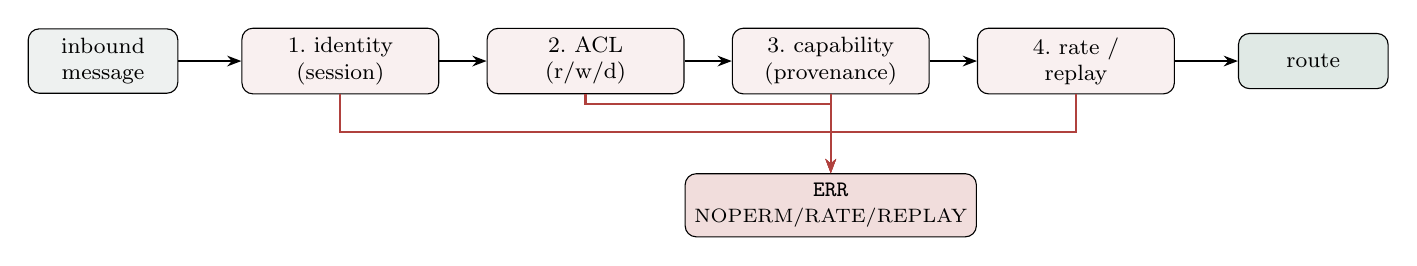
\begin{tikzpicture}[font=\footnotesize, node distance=7mm,
  chk/.style={draw, rounded corners, fill=tred!8, minimum width=2.5cm, minimum height=0.8cm, align=center},
  term/.style={draw, rounded corners, minimum width=1.9cm, minimum height=0.7cm, align=center},
  arr/.style={-{Stealth[length=1.8mm]}, thick}]
\node[term, fill=tgray] (in) {inbound\\ message};
\node[chk, right=8mm of in] (id) {1.~identity\\ (session)};
\node[chk, right=6mm of id] (acl) {2.~ACL\\ (r/w/d)};
\node[chk, right=6mm of acl] (cap) {3.~capability\\ (provenance)};
\node[chk, right=6mm of cap] (rr) {4.~rate /\\ replay};
\node[term, right=8mm of rr, fill=tgreen!15] (ok) {route};
\node[term, below=10mm of cap, fill=tred!18] (no) {\texttt{ERR}\\ \scriptsize NOPERM/RATE/REPLAY};
\draw[arr] (in)--(id); \draw[arr] (id)--(acl); \draw[arr] (acl)--(cap); \draw[arr] (cap)--(rr); \draw[arr] (rr)--(ok);
\draw[arr, tred] (id) -- ++(0,-0.9) -| (no);
\draw[arr, tred] (acl) -- ++(0,-0.55) -| (no);
\draw[arr, tred] (cap) -- (no);
\draw[arr, tred] (rr) -- ++(0,-0.9) -| (no);
\end{tikzpicture}
\caption{Broker-side security filter. Every inbound message passes four ordered checks; any failure
short-circuits to a typed error and is never routed. Identity is derived from the session (never the
wire); the capability check refuses, e.g., \texttt{EXEC}/\texttt{PAY}/\texttt{DELETE} on user-origin
content.}
\label{fig:security}
\end{figure}

\subsubsection{Broker / router}\label{sec:arch:broker}
The broker is where routing and identity meet, and two design decisions there carry most of the weight.
The first is \emph{identity by session}. When an agent connects, it completes a SYN/ACK handshake and
the broker binds one \texttt{agent\_id} to that connection for its lifetime; from then on, ``who sent
this'' is read from the connection, not from any field the sender can write. In the trace
(Figure~\ref{fig:trace}, step~2) the broker stamps \texttt{orchestrator} on the request itself ---
there is simply no place in the wire frame for a sender to claim otherwise. This is the structural
reason a compromised agent cannot impersonate another: spoofing would require hijacking the TCP session,
not just editing a string.

The second is \emph{correlation by \texttt{msg\_id} rather than by reply-to address}. The requester
chooses an id (8 in the trace); the broker remembers that id $\to$ requester mapping, forwards the
request to the target, and when a \texttt{RES} or \texttt{ERR} comes back carrying the same id, it
delivers it to whoever originally sent id 8. The worker therefore replies \emph{to the id}, never to
``the orchestrator''; it never has to know, and so can never forge, the requester's identity. This also
makes concurrency safe for free: an agent can have many requests in flight and the broker untangles the
replies by id, so two overlapping summaries cannot get crossed. The same machinery drives
subscriptions: a \texttt{PATCH} (a \texttt{DLT} message) to a context fans out an \texttt{EVT} to every
agent that subscribed to it, which is how collaborative state changes propagate without polling.
Figure~\ref{fig:broker} shows both mechanisms side by side.

Routing everything through one broker is what makes all of this possible, and it is also the system's
main structural weakness: the broker is a single point of failure and a throughput chokepoint. We state
that plainly as a threat-model assumption rather than design around it here (\S\ref{sec:disc}); making
the broker highly available is exactly the distributed-systems work we have not done.

\begin{figure}[h]\centering
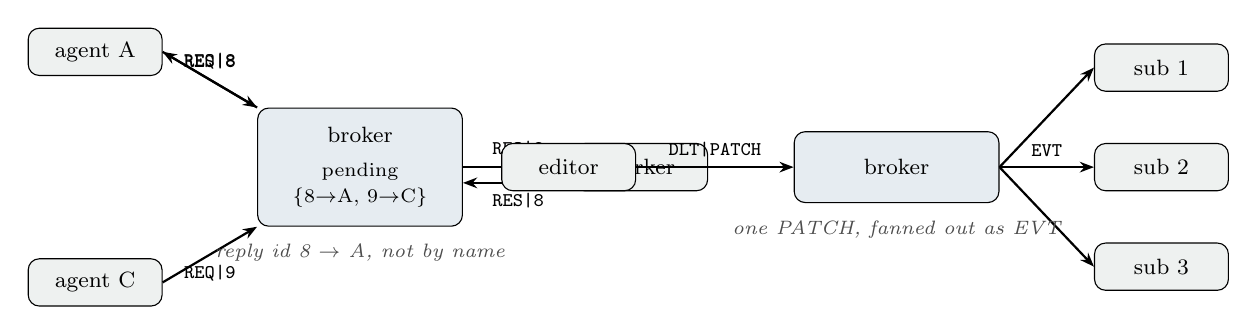
\begin{tikzpicture}[font=\footnotesize, node distance=5mm,
  ag/.style={draw, rounded corners, fill=tgray, minimum width=1.7cm, minimum height=0.6cm},
  brk/.style={draw, rounded corners, fill=tblue!12, minimum width=2.6cm, minimum height=1.5cm, align=center},
  arr/.style={-{Stealth[length=1.8mm]}, thick}]
% left: correlation
\node[brk] (b1) {broker\\[1mm]\scriptsize pending\\\scriptsize \{8$\to$A, 9$\to$C\}};
\node[ag, above left=4mm and 12mm of b1] (a) {agent A};
\node[ag, below left=4mm and 12mm of b1] (c) {agent C};
\node[ag, right=14mm of b1] (w) {worker};
\draw[arr] (a.east) -- node[above,font=\scriptsize]{\ttfamily REQ|8} (b1.north west);
\draw[arr] (c.east) -- node[below,font=\scriptsize]{\ttfamily REQ|9} (b1.south west);
\draw[arr] (b1.east) -- node[above,font=\scriptsize]{\ttfamily REQ|8} (w.west);
\draw[arr] ($(w.west)+(0,-2mm)$) -- node[below,font=\scriptsize]{\ttfamily RES|8} ($(b1.east)+(0,-2mm)$);
\draw[arr] (b1.north west) -- node[above,font=\scriptsize]{\ttfamily RES|8} (a.east);
\node[font=\scriptsize\itshape, gray!60!black, below=1mm of b1] {reply id 8 $\to$ A, not by name};
% right: fan-out
\node[brk, right=42mm of b1, minimum height=0.9cm] (b2) {broker};
\node[ag, left=20mm of b2] (e) {editor};
\node[ag, above right=5mm and 12mm of b2] (s1) {sub 1};
\node[ag, right=12mm of b2] (s2) {sub 2};
\node[ag, below right=5mm and 12mm of b2] (s3) {sub 3};
\draw[arr] (e.east) -- node[above,font=\scriptsize]{\ttfamily DLT|PATCH} (b2.west);
\draw[arr] (b2.east) -- node[font=\scriptsize]{} (s1.west);
\draw[arr] (b2.east) -- node[above,font=\scriptsize]{\ttfamily EVT} (s2.west);
\draw[arr] (b2.east) -- node[font=\scriptsize]{} (s3.west);
\node[font=\scriptsize\itshape, gray!60!black, below=1mm of b2] {one PATCH, fanned out as EVT};
\end{tikzpicture}
\caption{Two broker mechanisms. \emph{Left:} correlation by \texttt{msg\_id} --- the broker holds a
pending map (id $\to$ requester) so concurrent requests from A and C are untangled, and a worker's
\texttt{RES|8} is returned to A by its id, never by a name the worker had to know. \emph{Right:}
subscription fan-out --- a single \texttt{PATCH} to a context is pushed as an \texttt{EVT} to every
subscriber, so collaborative changes propagate without polling.}
\label{fig:broker}
\end{figure}

\subsubsection{Shared context store}\label{sec:arch:store}
This is where the document in the trace actually lives. Content is written once and addressed by a
numeric id (\texttt{CTX:42}), and an entry is more than its bytes: it carries the broker-derived owner,
an ACL, the capability provenance the security layer reads, a TTL with lazy and swept garbage
collection, a monotonic version with an append-only field-level delta log, and the set of subscribers
to notify on change. Each piece of that metadata earns a property the bare bytes could not give. Storing
the content (rather than a digest of it) is what makes a reference \emph{lossless} --- the worker that
resolves \texttt{CTX:42} sees the original document, so nothing is silently dropped, which is the whole
point established in \S\ref{sec:lossless}. Carrying provenance \emph{with} the entry is what lets the
security check travel with the reference instead of being re-derived at each hop. And the version plus
delta log is what makes a context safe to \emph{edit} collaboratively: a \texttt{PATCH} appends a
versioned delta and wakes subscribers, rather than two agents clobbering each other's writes. The
backend today is in-memory and single-node, which is enough to demonstrate all of this but not to
survive a restart or scale across machines; a durable, distributed store is future work
(\S\ref{sec:future}), and is the honest precondition for the systematization argument.
Figure~\ref{fig:entry} lays out one entry and what each field buys.

\begin{figure}[h]\centering
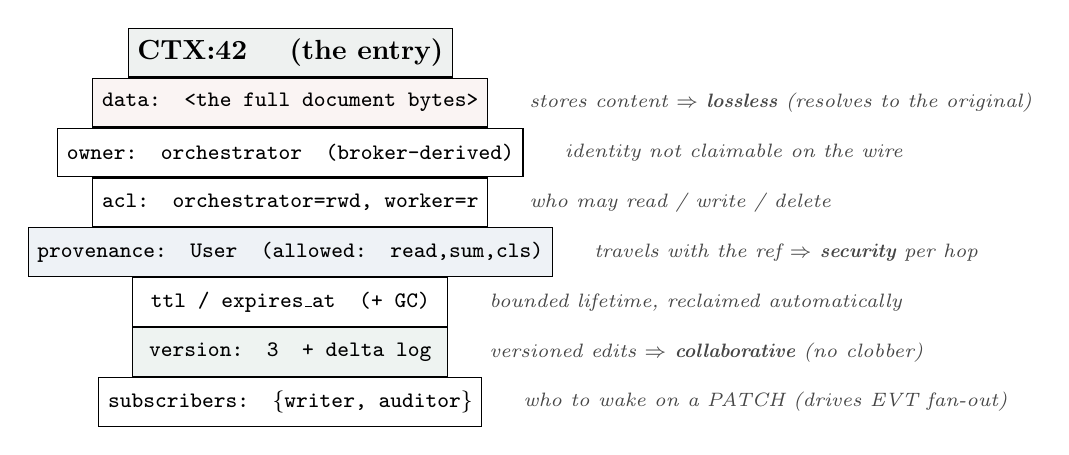
\begin{tikzpicture}[font=\footnotesize, node distance=0mm,
  field/.style={draw, minimum width=4.0cm, minimum height=0.62cm, anchor=north, align=left},
  prop/.style={font=\scriptsize\itshape, gray!55!black, anchor=west},
  arr/.style={-{Stealth[length=1.6mm]}, gray!60}]
\node[field, fill=tgray, font=\bfseries] (h) {CTX:42 \quad (the entry)};
\node[field, fill=tred!6, below=0mm of h] (data) {\ttfamily data: <the full document bytes>};
\node[field, below=0mm of data] (owner) {\ttfamily owner: orchestrator \ (broker-derived)};
\node[field, below=0mm of owner] (acl) {\ttfamily acl: orchestrator=rwd, worker=r};
\node[field, fill=tblue!8, below=0mm of acl] (prov) {\ttfamily provenance: User \ (allowed: read,sum,cls)};
\node[field, below=0mm of prov] (ttl) {\ttfamily ttl / expires\_at \ (+ GC)};
\node[field, fill=tgreen!8, below=0mm of ttl] (ver) {\ttfamily version: 3 \ + delta log};
\node[field, below=0mm of ver] (subs) {\ttfamily subscribers: \{writer, auditor\}};
% property annotations
\node[prop] at ($(data.east)+(4mm,0)$) {stores content $\Rightarrow$ \textbf{lossless} (resolves to the original)};
\node[prop] at ($(owner.east)+(4mm,0)$) {identity not claimable on the wire};
\node[prop] at ($(acl.east)+(4mm,0)$) {who may read / write / delete};
\node[prop] at ($(prov.east)+(4mm,0)$) {travels with the ref $\Rightarrow$ \textbf{security} per hop};
\node[prop] at ($(ttl.east)+(4mm,0)$) {bounded lifetime, reclaimed automatically};
\node[prop] at ($(ver.east)+(4mm,0)$) {versioned edits $\Rightarrow$ \textbf{collaborative} (no clobber)};
\node[prop] at ($(subs.east)+(4mm,0)$) {who to wake on a PATCH (drives EVT fan-out)};
\end{tikzpicture}
\caption{Anatomy of a stored context. The entry is far more than its bytes; each field earns a property
the bare content could not. Storing the content (not a digest) is what makes the reference lossless;
carrying provenance \emph{in} the entry is what lets security travel with it; the version and delta log
are what make collaborative edits safe.}
\label{fig:entry}
\end{figure}

\subsubsection{Transport}\label{sec:arch:transport}
The bottom layer just moves bytes: length-prefixed records over TCP (Tokio), where the prefix tells the
reader how many bytes to expect so messages can be reassembled from a stream without a delimiter that
could collide with payload data. We keep this layer deliberately dumb and free of protocol knowledge,
so that swapping in WebSocket or gRPC later changes nothing above it. Nothing in the agent, protocol,
security, or broker layers depends on the transport choice.

\begin{figure}[h]\centering
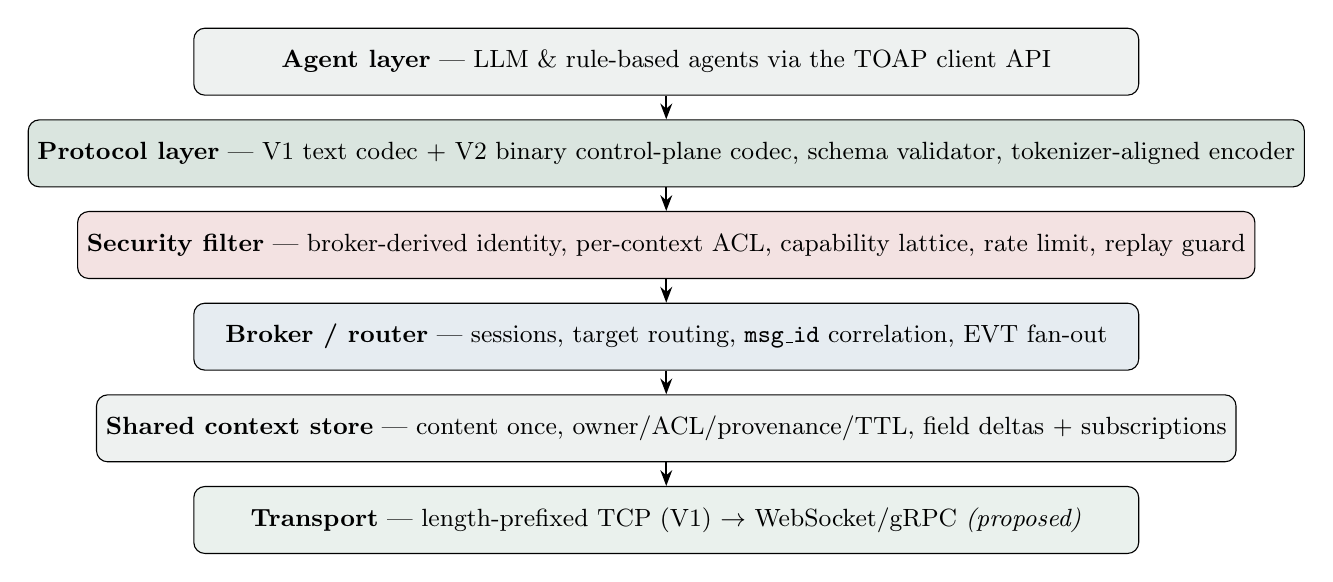
\begin{tikzpicture}[font=\small, node distance=3mm,
  layer/.style={draw, rounded corners, minimum width=12cm, minimum height=0.85cm, align=center},
  arr/.style={-{Stealth[length=2mm]}, thick}]
\node[layer, fill=tgray] (ag) {\textbf{Agent layer} --- LLM \& rule-based agents via the TOAP client API};
\node[layer, fill=tgreen!18, below=of ag] (pr) {\textbf{Protocol layer} --- V1 text codec + V2 binary control-plane codec, schema validator, tokenizer-aligned encoder};
\node[layer, fill=tred!15, below=of pr] (se) {\textbf{Security filter} --- broker-derived identity, per-context ACL, capability lattice, rate limit, replay guard};
\node[layer, fill=tblue!12, below=of se] (br) {\textbf{Broker / router} --- sessions, target routing, \texttt{msg\_id} correlation, EVT fan-out};
\node[layer, fill=tgray, below=of br] (cs) {\textbf{Shared context store} --- content once, owner/ACL/provenance/TTL, field deltas + subscriptions};
\node[layer, fill=tgreen!10, below=of cs] (tr) {\textbf{Transport} --- length-prefixed TCP (V1) $\rightarrow$ WebSocket/gRPC \emph{(proposed)}};
\draw[arr] (ag)--(pr); \draw[arr] (pr)--(se); \draw[arr] (se)--(br); \draw[arr] (br)--(cs); \draw[arr] (cs)--(tr);
\end{tikzpicture}
\caption{TOAP layered architecture. Identity/trust are broker-owned, never claimed on the wire.}
\label{fig:arch}
\end{figure}

\subsection{Two-plane wire format}\label{sec:twoplane}
A single message is read by two parties with opposite cost functions. The \emph{broker} needs ids,
session, ACL, capability tags, and nonces --- metadata whose cost is \emph{bytes} (bandwidth, parse
latency, framing) and which the LLM should never see. The \emph{LLM} needs the operation and its
content --- text whose cost is \emph{tokens} and which the broker should never tokenize. TOAP encodes
these as two planes: a compact binary \emph{control plane} optimized for bytes, and a
tokenizer-aligned \emph{semantic plane} optimized for tokens (Figure~\ref{fig:twoplane}). Because each
plane is encoded for its single reader, neither is dominated --- which is precisely why ``bytes vs.\
tokens'' (\S\ref{sec:bytes}) stops being a confusion: they are different planes with different objectives.

\begin{figure}[h]\centering
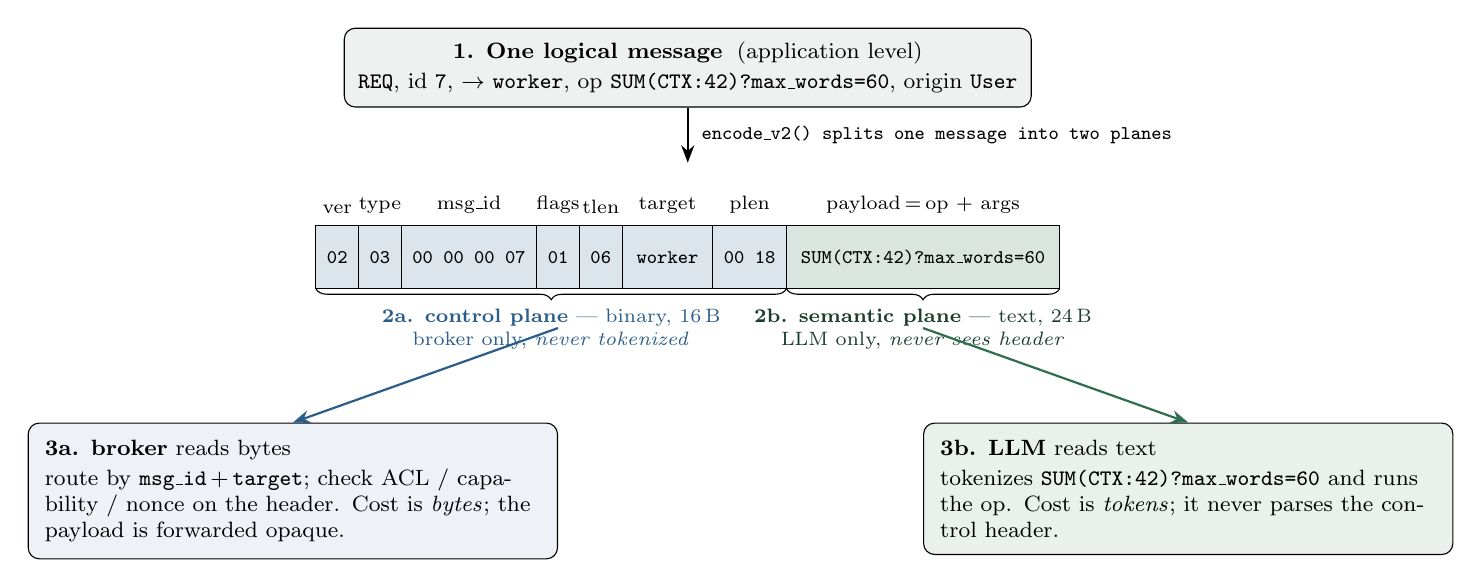
\begin{tikzpicture}[font=\footnotesize,
  cc/.style={draw, fill=tblue!16, minimum height=8mm, align=center, font=\ttfamily\scriptsize, inner xsep=4pt, outer sep=0pt},
  sc/.style={draw, fill=tgreen!18, minimum height=8mm, align=center, font=\ttfamily\scriptsize, inner xsep=4pt, outer sep=0pt},
  rd/.style={draw, rounded corners, align=left, inner sep=6pt, text width=6.3cm},
  arr/.style={-{Stealth[length=2.2mm]}, thick},
  lab/.style={font=\scriptsize}]

% --- the byte frame, built left-to-right (centerpiece) ---
\node[cc] (b0) at (0,0) {02};
\node[cc, right=0pt of b0] (b1) {03};
\node[cc, right=0pt of b1] (b2) {00 00 00 07};
\node[cc, right=0pt of b2] (b3) {01};
\node[cc, right=0pt of b3] (b4) {06};
\node[cc, right=0pt of b4] (b5) {\,worker\,};
\node[cc, right=0pt of b5] (b6) {00 18};
\node[sc, right=0pt of b6] (p)  {\,SUM(CTX:42)?max\_words=60\,};

% field labels above each cell
\node[lab, above=1pt of b0]{ver}; \node[lab, above=1pt of b1]{type};
\node[lab, above=1pt of b2]{msg\_id}; \node[lab, above=1pt of b3]{flags};
\node[lab, above=1pt of b4]{tlen}; \node[lab, above=1pt of b5]{target};
\node[lab, above=1pt of b6]{plen}; \node[lab, above=1pt of p]{payload\,=\,op + args};

% --- input message, centered above the frame ---
\node[draw, rounded corners, fill=tgray, align=center, inner sep=5pt, anchor=south]
  (in) at ($(b0.north west)!0.5!(p.north east)+(0,15mm)$)
  {\textbf{1. One logical message} \;(application level)\\[0.5mm]
   \texttt{REQ}, id \texttt{7}, $\to$ \texttt{worker}, op \texttt{SUM(CTX:42)?max\_words=60}, origin \texttt{User}};
\draw[arr] (in.south) -- node[right, lab]{\ttfamily\,encode\_v2() splits one message into two planes} ($(in.south)+(0,-7mm)$);

% --- braces under the frame marking the two planes ---
\draw[decorate, decoration={brace, amplitude=4pt, mirror}] (b0.south west) -- (b6.south east)
  node[midway, below=4pt, lab, tblue, align=center]
  {\textbf{2a. control plane} — binary, 16\,B\\ broker only, \emph{never tokenized}};
\draw[decorate, decoration={brace, amplitude=4pt, mirror}] (p.south west) -- (p.south east)
  node[midway, below=4pt, lab, tgreen!55!black, align=center]
  {\textbf{2b. semantic plane} — text, 24\,B\\ LLM only, \emph{never sees header}};

% --- two readers, each fed by its own plane ---
\node[rd, fill=tblue!8, anchor=north east] (br) at ($(b3.south)+(0,-1.7cm)$)
  {\textbf{3a. broker} reads bytes\\[0.5mm]
   route by \texttt{msg\_id}\,+\,\texttt{target}; check ACL / capability / nonce on the header.
   Cost is \emph{bytes}; the payload is forwarded opaque.};
\node[rd, fill=tgreen!10, anchor=north west] (llm) at ($(p.south)+(0,-1.7cm)$)
  {\textbf{3b. LLM} reads text\\[0.5mm]
   tokenizes \texttt{SUM(CTX:42)?max\_words=60} and runs the op. Cost is \emph{tokens}; it never
   parses the control header.};
\draw[arr, tblue]  ($(b3.south)+(0,-0.5cm)$) -- (br.north);
\draw[arr, tgreen] ($(p.south)+(0,-0.5cm)$)  -- (llm.north);
\end{tikzpicture}
\caption{How one message travels through the two planes (input $\to$ output). A single application-level
message is serialized by \texttt{encode\_v2()} into one frame holding two regions encoded for opposite
cost functions: a compact \emph{binary control plane} (version, type, \texttt{msg\_id}, flags, target,
length --- the only part the broker reads, and it never tokenizes it) followed by the \emph{text
semantic plane} (the \texttt{OP(args)?opts} the LLM reads and tokenizes, and never the header). Bytes
shown are the real \texttt{toap-core} V2 layout for this message. Because each region is optimized for
its single reader, neither is dominated --- which is why ``bytes vs.\ tokens'' (\S\ref{sec:bytes}) is a
plane distinction, not a confusion.}
\label{fig:twoplane}
\end{figure}

\subsection{Capability-lattice provenance}\label{sec:arch:security:cap}
A boolean ``tainted'' flag cannot express \emph{what} untrusted content may do. TOAP attaches a
provenance to each context: an \texttt{Origin} (\textsc{Internal}/\textsc{External}/\textsc{User}) and
the set of \texttt{Capability} values that origin permits (read, summarize, transform, classify,
execute, email, pay, delete). Trusted internal content permits all; external content permits read-only
flows (read/summarize/transform/classify) but no side effects; user-originated content is most
restricted. The broker maps each opcode to a capability (\texttt{Capability::for\_op}) and refuses any
operation the provenance forbids --- e.g.\ an \texttt{EXEC}/\texttt{PAY}/\texttt{DELETE} driven by
user-origin content returns \texttt{NOPERM reason=capability\_denied}. Because the tag travels with the
reference, taint is preserved across agent-to-agent hops, structurally containing prompt-injection
propagation rather than relying on fragile content pattern-matching.

\subsection{Reference materialization spectrum}\label{sec:refspec}
``Send the text,'' ``send a context id,'' and ``send a KV-cache pointer'' are not three features but
three \emph{materializations of one logical reference}, chosen per call by a cost model and degrading
gracefully when constraints fail: \textsc{KV\_Bridge}~$\rightarrow$~\textsc{Ctx\_Ref}~$\rightarrow$
\textsc{Inline}. \textsc{Inline} embeds the bytes (best for tiny/one-shot content); \textsc{Ctx\_Ref}
sends the id and the receiver fetches from the store (the dedup win for reused content); \textsc{KV\_Bridge}
points at a reusable KV cache so the receiver skips prefill (valid only for the same model and
tokenizer). The same decision --- materialize now vs.\ reference vs.\ reuse computation --- spans both
the token plane (resend text vs.\ send id) and the tensor plane (re-prefill vs.\ load KV); treating
them as one policy is the architecture's most novel point (Figure~\ref{fig:spectrum}).
Figure~\ref{fig:flow} shows the token-flow contrast the experiment measures: naive prompts grow with
pipeline depth while references stay flat, because the store holds content once and only ids travel.

\begin{figure}[h]\centering
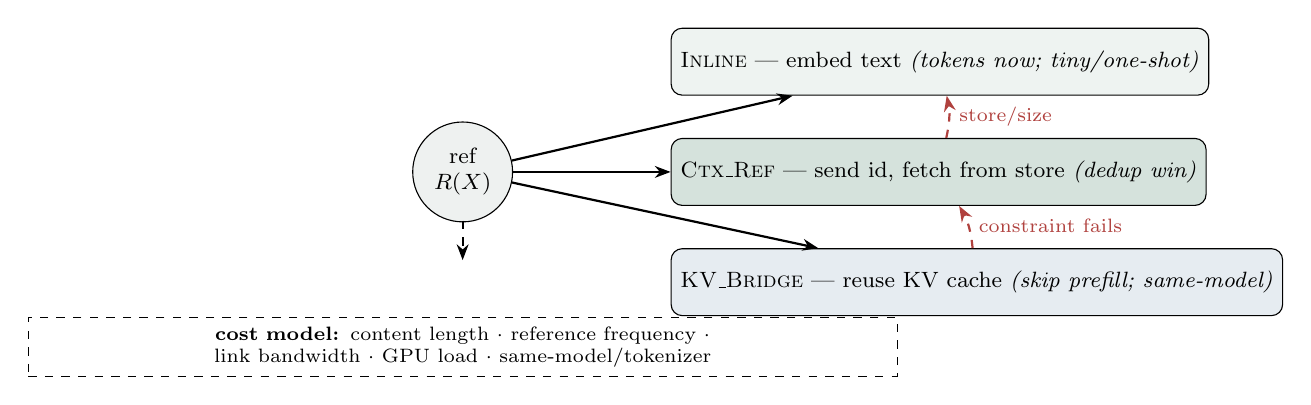
\begin{tikzpicture}[font=\footnotesize, node distance=6mm,
  ref/.style={draw, circle, fill=tgray, minimum size=1.15cm, align=center},
  opt/.style={draw, rounded corners, minimum width=5.6cm, minimum height=0.85cm, align=center},
  arr/.style={-{Stealth[length=2mm]}, thick}]
\node[ref] (r) {ref\\ $R(X)$};
\node[opt, fill=tgreen!8,  right=20mm of r, yshift=14mm] (i) {\textsc{Inline} --- embed text \emph{(tokens now; tiny/one-shot)}};
\node[opt, fill=tgreen!20, right=20mm of r]              (c) {\textsc{Ctx\_Ref} --- send id, fetch from store \emph{(dedup win)}};
\node[opt, fill=tblue!12,  right=20mm of r, yshift=-14mm] (k) {\textsc{KV\_Bridge} --- reuse KV cache \emph{(skip prefill; same-model)}};
\draw[arr] (r)--(i); \draw[arr] (r)--(c); \draw[arr] (r)--(k);
% graceful-degradation chain
\draw[arr, tred, dashed] (k) to[bend right=12] node[right, font=\scriptsize, tred]{constraint fails} (c);
\draw[arr, tred, dashed] (c) to[bend right=12] node[right, font=\scriptsize, tred]{store/size} (i);
\node[draw, dashed, below=12mm of r, text width=10.8cm, align=center, font=\scriptsize]
  {\textbf{cost model:} content length $\cdot$ reference frequency $\cdot$ link bandwidth $\cdot$ GPU load $\cdot$ same-model/tokenizer};
\draw[arr, dashed] ($(r)+(0,-0.62)$) -- ++(0,-0.5);
\end{tikzpicture}
\caption{Reference materialization spectrum: one logical reference, three materializations chosen per
call by a cost model, with graceful degradation
$\textsc{KV\_Bridge}\!\rightarrow\!\textsc{Ctx\_Ref}\!\rightarrow\!\textsc{Inline}$ when constraints
fail. The same decision spans the token plane (resend vs.\ id) and the tensor plane (re-prefill vs.\
load KV).}
\label{fig:spectrum}
\end{figure}

\begin{figure}[h]\centering
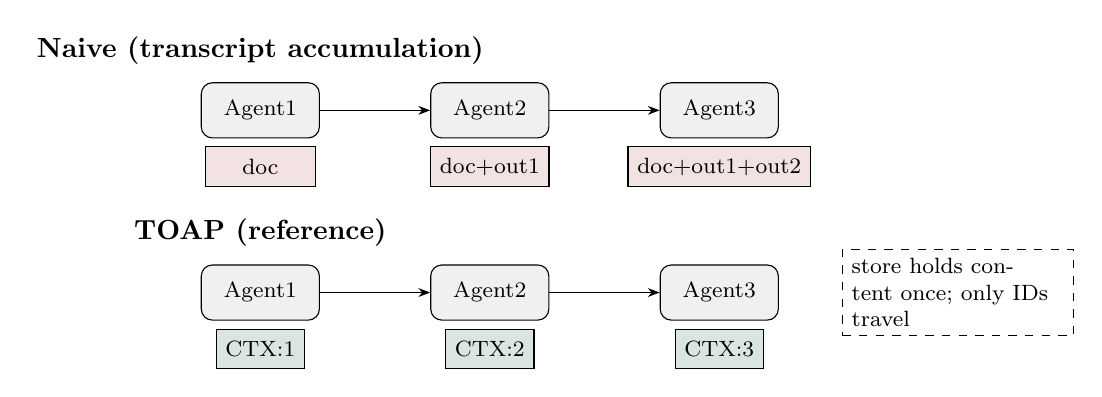
\begin{tikzpicture}[font=\footnotesize, node distance=5mm,
  ag/.style={draw, rounded corners, fill=tgray, minimum width=1.5cm, minimum height=0.7cm},
  doc/.style={draw, fill=tred!15, minimum width=1.4cm, minimum height=0.5cm},
  ref/.style={draw, fill=tgreen!18, minimum width=1.0cm, minimum height=0.5cm}]
% naive row
\node[ag] (a1) {Agent1}; \node[ag, right=14mm of a1] (a2) {Agent2}; \node[ag, right=14mm of a2] (a3) {Agent3};
\node[above=1mm of a1, font=\bfseries] {Naive (transcript accumulation)};
\node[doc, below=1mm of a1] (d1) {doc}; \node[doc, below=1mm of a2] (d2) {doc+out1}; \node[doc, below=1mm of a3] (d3) {doc+out1+out2};
\draw[-{Stealth[length=1.5mm]}] (a1)--(a2); \draw[-{Stealth[length=1.5mm]}] (a2)--(a3);
% toap row
\node[ag, below=16mm of a1] (b1) {Agent1}; \node[ag, right=14mm of b1] (b2) {Agent2}; \node[ag, right=14mm of b2] (b3) {Agent3};
\node[above=1mm of b1, font=\bfseries] {TOAP (reference)};
\node[ref, below=1mm of b1] (r1) {CTX:1}; \node[ref, below=1mm of b2] (r2) {CTX:2}; \node[ref, below=1mm of b3] (r3) {CTX:3};
\draw[-{Stealth[length=1.5mm]}] (b1)--(b2); \draw[-{Stealth[length=1.5mm]}] (b2)--(b3);
\node[draw, dashed, right=8mm of b3, text width=2.7cm] {store holds content once; only IDs travel};
\end{tikzpicture}
\caption{Token-flow contrast: naive prompts grow with depth; references stay flat.}
\label{fig:flow}
\end{figure}

\subsection{Implemented vs.\ proposed}\label{sec:arch:status}
\callout{\textbf{Implemented today} (29 passing unit + integration tests): the V1 text protocol and
parser; the \textbf{V2 binary control plane} (compact binary control header + text semantic payload ---
the two-plane design, with round-trip tests); the shared context store with per-context ACL, TTL,
field-level deltas, and subscriptions; a \textbf{capability-lattice} provenance model (Origin $\in$
\{Internal, External, User\}, each with an allowed-capability set) the broker enforces structurally
(user-/external-origin content cannot flow into EXEC/PAY/DELETE); an \textbf{in-band cache coordinate}
with a stable-prefix~$\|$~volatile-suffix layout helper; the \textbf{materialization policy with
graceful fallback} (KV\_BRIDGE~$\rightarrow$~CTX\_REF~$\rightarrow$~INLINE) behind a \texttt{KvTransport}
trait; broker-derived identity, token-bucket rate limiting, per-session replay rejection,
\texttt{msg\_id} correlation; and an MCP frontend.\\[1mm]
A minimal \textbf{KV-cache transport} is now implemented as a same-model, same-tokenizer
\emph{prefix-reuse} sidecar (\texttt{benchmark/kv\_bridge}): it extracts a shared context's KV,
serializes/transfers it, and lets the receiver prefill only its query suffix, with a benchmark that
measures prefill-latency saved, KV-byte-size vs.\ text-size, and exact greedy-output correctness. The
Rust side owns the policy and fallback (\texttt{RegistryKvTransport} enforces the same-model
constraint); the sidecar owns the tensor transport. We deliberately restrict to prefix reuse (absolute
positions preserved) and do \emph{not} splice caches across positions. Cross-vendor evaluation remains
future work.}

\section{Implementation}\label{sec:impl}
TOAP is a Rust workspace. \texttt{toap-core} defines the message model, a strict recursive-descent
parser, and the encoder; it deliberately rejects malformed \emph{protocol} syntax but never rejects
ordinary content for ``looking dangerous'' (SQL/HTML/prompt-like text are data). \texttt{toap-context}
implements the in-memory store: numeric context IDs, an ACL grammar (\texttt{agent:rwd}), a
\emph{capability-lattice} provenance model (\texttt{Origin} $\times$ allowed \texttt{Capability} set,
with \texttt{Capability::for\_op} mapping opcodes to capabilities), TTL with lazy + sweep GC, a bounded
per-context delta log, the \texttt{Reference} materialization enum with a
\texttt{materialize\_with\_fallback} policy behind a \texttt{KvTransport} trait, and a
\texttt{cache\_layout} helper for stable-prefix ordering. \texttt{toap-core} also provides a V2 binary
control-plane codec (\texttt{encode\_v2}/\texttt{decode\_v2}) that round-trips the V1 message model.
\texttt{toap-security} provides a token-bucket rate limiter and a per-session replay guard; the broker
enforces the capability lattice structurally, refusing e.g.\ an
\texttt{EXEC}/\texttt{PAY}/\texttt{DELETE} against user- or external-origin context. \texttt{toap-broker} is an asynchronous (Tokio) TCP server with length-prefixed
framing; identity is bound to the connection at SYN, and a responder addresses replies by the original
\texttt{msg\_id} so it never learns the requester (preventing source spoofing). \texttt{toap-client}
is an async SDK; \texttt{toap-mcp} is the MCP frontend.

Testing is unit \emph{and} integration: parser round-trip/validation and store/ACL/TTL/delta unit
tests, plus end-to-end integration tests in which \textbf{real client processes connect to the broker
over TCP} and exchange requests --- the broker performs actual routing and store operations (not
mocked). Security integration tests assert that an unauthorized read is denied, a restricted op on
tainted context is refused, and a subscriber receives a delta event. A live multi-process demo
(broker + summarizer + classifier + orchestrator) exercises fan-out and merge. Coordination-frame
sizes reported below are measured on the actual encoder output.

\section{Why a Protocol, Not Just a Better Orchestrator?}\label{sec:why}
The sharpest objection is: ``just write an orchestrator that summarizes before forwarding.'' Our token
experiment confirms a summarizing orchestrator is in fact \emph{more} token-efficient than referencing
(\S\ref{sec:results}), so the case for a protocol cannot rest on token savings. It rests on two
properties a prompt-engineering pattern does not provide, and we point to the measurement for each
rather than asserting them. \textbf{(i) Losslessness.} A reference can be re-expanded on demand; a
summary discards information irreversibly. This is not hypothetical: when the discarded detail is the
one a downstream step needs, the summary arm fails and the reference arm does not (8/8 vs.\ 6/8,
\S\ref{sec:lossless}). \textbf{(ii) Security travels with the reference.} Provenance and broker-derived
identity are enforced structurally, so untrusted content cannot be laundered into a side-effecting
operation regardless of how the injection is phrased --- 40/40 attempts blocked at no cost to benign
traffic (\S\ref{sec:security-eval}); a summarizing prompt template offers none of this. A third
intended property, \emph{systematization} across heterogeneous agents, is a design goal of the protocol
but is not something this paper measures (the implementation is single-language and single-node); we
list it as motivation, not as a result. The honest bottom line is that referencing earns its place in
exactly the regimes where losslessness or in-band security matters, and yields to summarization where
neither does.

\section{Experimental Method}\label{sec:method}
\textbf{Instrument.} Each agent call is an isolated Claude subagent at an explicit model
(Haiku/Sonnet/Opus), tool use disabled; outputs are genuine generations.
\textbf{Controlled design.} To get clean variance we fix one canonical upstream (one document, one
extracted-facts text, and one analysis containing all four rubric themes) so the only variables are
\{model, context strategy, sample\}. Three strategies for the final \emph{writer} stage:
\emph{naive} (document + facts + analysis), \emph{summary} (a short lossy summary of the analysis,
i.e.\ a competent summarizing orchestrator), and \emph{TOAP} (the analysis only, i.e.\ the distilled
slice passed by reference). We draw $n{=}5$ samples per cell for Haiku and $n{=}3$ for Sonnet/Opus
($n{=}33$ total).
\textbf{Accuracy (bias-free).} The primary accuracy measure is a \emph{deterministic} rubric checker:
each of four required actions is detected by keyword sets, with no model in the loop, so it is immune
to same-family judge bias and exactly reproducible. (A model judge was used only in an earlier
single-sample run and is not relied upon here.)
\textbf{Tokens.} Counted with \texttt{tiktoken} (cl100k) on the exact prompts and verbatim outputs.
\textbf{Reproducibility.} All prompts, verbatim outputs, and the scorer are committed.

\callout{\textbf{Reviewer-driven changes.} A first review noted the token study was thin; a second
noted that the paper disproved its headline without establishing its replacement. In response we
(1) replaced $n{=}1$ with $n{=}33$ and added a \emph{strong} summarizing baseline; (2) switched to a
deterministic, model-independent scorer; (3) \emph{ran} the losslessness experiment the earlier draft
had only named as missing (\S\ref{sec:lossless}); (4) added an adversarial evaluation of the capability
lattice (\S\ref{sec:security-eval}); and (5) implemented and measured KV transfer across seven models
(\S\ref{sec:kv-results}). The single-model-family scope of the token study remains, and we ship a
notebook to retire it (\S\ref{sec:lossless}).}

\section{Results}\label{sec:results}
\textbf{Accuracy parity; the regression retracted.} All 33 samples scored 4/4 on the deterministic
rubric (Figure~\ref{fig:parity}); coverage variance was zero. A 4/4$\rightarrow$3/4 Haiku regression
seen in an earlier \emph{single-sample} run \textbf{did not reproduce} at $n{=}5$ with a fixed upstream;
we attribute it to single-sample noise and/or propagation of a weaker upstream analysis, and retract it.

\textbf{Tokens: the summarizing baseline beats TOAP.} Table~\ref{tab:writer} and
Figure~\ref{fig:threearm} give total writer tokens. Against the naive baseline, TOAP cuts tokens by
1.88--1.93$\times$ (mean $\sim$1.91$\times$); the summarizing baseline cuts them by 2.39--2.62$\times$
(mean $\sim$2.54$\times$). Both hold 4/4 accuracy. Reference-passing, in other words, is not the most
token-efficient strategy; a competent summarizer is. We state this plainly because it is the result
most likely to be glossed over, and because it reframes what the rest of the protocol is for.

\begin{table}[h]\centering\footnotesize
\begin{tabular}{llcccc}
\toprule
Model & Strategy & $n$ & Accuracy (/4) & Total tokens (mean [min--max]) & Reduction vs.\ naive \\
\midrule
Haiku  & naive   & 5 & 4.0 & 505 [491--520] & --- \\
Haiku  & summary & 5 & 4.0 & 211 [193--219] & 2.39$\times$ \\
Haiku  & TOAP    & 5 & 4.0 & 268 [258--279] & 1.88$\times$ \\
Sonnet & naive   & 3 & 4.0 & 512 [499--523] & --- \\
Sonnet & summary & 3 & 4.0 & 195 [190--204] & 2.62$\times$ \\
Sonnet & TOAP    & 3 & 4.0 & 266 [265--267] & 1.93$\times$ \\
Opus   & naive   & 3 & 4.0 & 504 [487--519] & --- \\
Opus   & summary & 3 & 4.0 & 194 [192--196] & 2.60$\times$ \\
Opus   & TOAP    & 3 & 4.0 & 263 [253--271] & 1.92$\times$ \\
\bottomrule
\end{tabular}
\caption{Controlled writer experiment ($n{=}33$). Accuracy by deterministic rubric (bias-free).
Tokens via tiktoken. TOAP $<$ naive, but summary $<$ TOAP.}
\label{tab:writer}
\end{table}

\begin{figure}[h]\centering
\begin{minipage}{0.49\textwidth}\centering
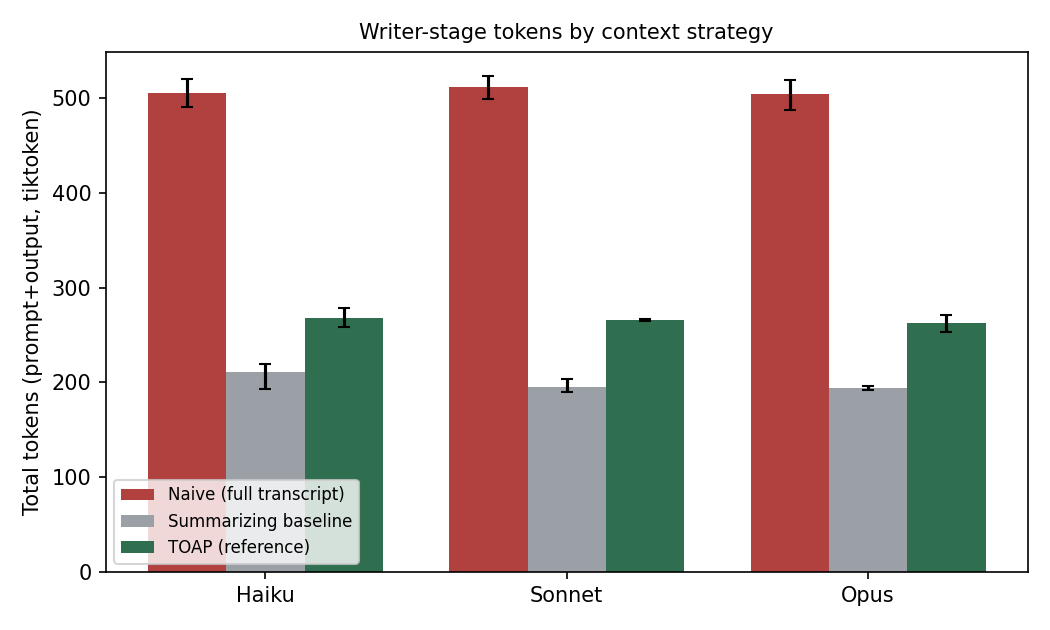
\includegraphics[width=\textwidth]{figures/fig_threearm.png}
\caption{Writer tokens by strategy (error = min--max). Summary $<$ TOAP $<$ naive.}\label{fig:threearm}
\end{minipage}\hfill
\begin{minipage}{0.49\textwidth}\centering
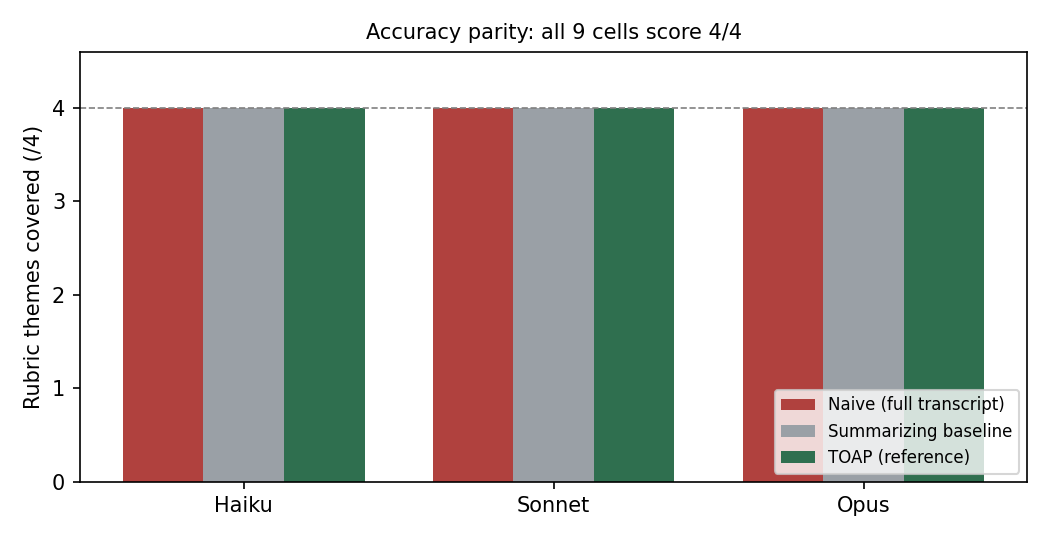
\includegraphics[width=\textwidth]{figures/fig_parity.png}
\caption{Accuracy parity: all nine cells 4/4 (the $n{=}1$ regression did not reproduce).}\label{fig:parity}
\end{minipage}
\end{figure}

\textbf{Where referencing does win: multi-hop and coordination.} The writer experiment is a single hop.
In a multi-hop pipeline, referencing avoids re-summarizing/re-sending at \emph{every} hop, and the
store's send-once/refer-many compounds; an exploratory three-stage run showed 1.65--1.82$\times$
downstream reductions. Separately, TOAP coordination frames are $\sim$17$\times$ smaller in tokens than
JSON-RPC equivalents (model-independent, exactly reproducible). These are the regimes where a reference
protocol, rather than per-hop summarization, is the natural fit --- and where losslessness matters most.

\subsection{Losslessness under pressure: when a summary's lossiness costs accuracy}\label{sec:lossless}
The token experiment above used an easy task on which every strategy reached 4/4, so it could not show
the cost of a summary's lossiness; that absence was the most important gap in an earlier draft. We
close it with a pre-registered experiment designed so that lossiness must bite. A 130-word incident
report carries eight distinct facts (a rollback time, a revenue figure, a PR number, the reason a bad
config passed staging, and so on). We had a summarizer subagent compress it faithfully to 45 words ---
a length at which all eight facts cannot survive --- and then asked a downstream responder eight fixed
questions, each needing one specific fact, under two conditions: \emph{summary} (it sees only the
45-word summary) and \emph{reference} (it sees the full document, i.e.\ the lossless reference
materialized). The scenario, questions, and ground-truth answers were fixed before any responder ran;
grading is deterministic substring matching; three samples per arm.

The faithful summary dropped two of the eight facts (the rollback time and the staging-schema reason).
The downstream consequence is exactly as predicted: the \textbf{reference arm scores 8/8} in all three
runs, while the \textbf{summary arm scores 6/8}, missing precisely the two questions whose facts were
dropped (Table~\ref{tab:lossless}). This is the empirical content of the losslessness claim: a summary
is cheaper (\S\ref{sec:results}) until a later step needs something it discarded, at which point it
fails silently; a reference cannot, because the information is still there to be re-read. It is a
single scenario on the Claude family and we do not generalize the magnitude, but the mechanism it
demonstrates is not Claude-specific --- any lossy compression of $k$ facts into fewer than $k$ will
drop some, and any task needing a dropped one will fail. We ship a notebook
(\texttt{benchmark/ab\_study/lossless/lossless\_colab.ipynb}) that re-runs the identical pre-registered
experiment on an open instruct model (Qwen/Llama/Mistral) at $n{=}10$ per arm, so the one run that would
remove the single-family caveat for this claim is a button-press, not a rewrite.

\begin{table}[h]\centering\footnotesize
\begin{tabular}{lcc}
\toprule
Downstream question (fact needed) & Summary arm & Reference arm \\
\midrule
Pool ceiling value; revenue; PR \#; lower bound; alert threshold; runbook (6 facts) & 3/3 & 3/3 \\
Rollback time (09:51) --- \emph{dropped by summary} & \textbf{0/3} & 3/3 \\
Why staging passed (different schema) --- \emph{dropped by summary} & \textbf{0/3} & 3/3 \\
\midrule
\textbf{Total (mean of 3 runs)} & \textbf{6/8} & \textbf{8/8} \\
\bottomrule
\end{tabular}
\caption{Losslessness under pressure. A faithful 45-word summary of an 8-fact document drops two facts;
the downstream responder then fails exactly those two questions, while the lossless reference answers
all eight. Pre-registered; deterministic grading; \texttt{benchmark/ab\_study/lossless/}.}
\label{tab:lossless}
\end{table}

\subsection{Does the capability lattice actually stop anything?}\label{sec:security-eval}
\S\ref{sec:arch:security:cap} describes the lattice; the fair question is whether it stops real attacks
or is just plausible-looking infrastructure. We threw a corpus at it. The threat we model is a prompt
injection that tries to make untrusted content (User- or External-origin) drive a side-effecting
operation, and we cover nine flavours of it: straightforward exfiltration, code and shell execution,
payments, deletes, privilege escalation through writes, the same restricted call buried at the end of a
multi-hop chain, a payload assembled across several context updates, novel or mis-cased opcodes hoping
to slip past the dispatcher, and the same attacks dressed up in base64, Unicode homoglyphs, or
zero-width characters. That is 40 attacks in total, alongside 14 benign requests (reads, summaries,
classifications, and the legitimate transforms that External content is allowed). Each is sent through
the same broker check, which maps the requested opcode to a capability and refuses anything the
content's provenance does not permit. The lattice \textbf{blocked all 40 attacks and allowed all 14
benign requests} --- a 100\% block rate at a 0\% false-positive rate, the same in every category
(Table~\ref{tab:redteam}).

We are not claiming a clever detector here, and the chaining and obfuscation cases are in the corpus to
make that explicit: the decision is taken on (origin, capability), never on the text, so where the
injection sits in a chain or how it is encoded simply does not enter the computation. That is the
strength and also the boundary. A capability gate governs what untrusted content may be \emph{used
for}; it says nothing about attacks that live elsewhere. We include two such cases and confirm the
lattice does \emph{not} stop them, by design: an injection that stays inside an allowed capability (it
only asks for a summary, then steers that summary) sails through, and content whose origin was
mislabeled \textsc{Internal} at ingress is trusted on that label. Defending those needs output-side
checks and a trustworthy tagging boundary respectively --- separate components we assume rather than
evaluate. The whole corpus, the per-category counts, and the two boundary cases are a committed test
(\texttt{crates/toap-context/tests/capability\_redteam.rs}), so the result regenerates from a clean
checkout.

\begin{table}[h]\centering\footnotesize
\begin{tabular}{lc@{\hskip 2em}lc}
\toprule
Attack category & Blocked & Attack category & Blocked \\
\midrule
Exfiltration (email)      & 5/5 & Multi-hop chain        & 4/4 \\
Execution (exec/shell)    & 6/6 & Split payload          & 3/3 \\
Financial (pay)           & 4/4 & Stepping-stone opcode  & 4/4 \\
Destructive (delete)      & 4/4 & Obfuscation/encoding   & 5/5 \\
Escalation (write/xform)  & 5/5 & \textbf{All / benign}  & \textbf{40/40 \ \ 0 FP/14} \\
\bottomrule
\end{tabular}
\caption{Capability-lattice red team. 40 injection attempts across nine categories, all blocked; 14
benign read/analysis requests, none blocked. Two documented boundary cases (within-capability steering;
mislabeled origin) are \emph{not} blocked, by design.}
\label{tab:redteam}
\end{table}

\subsection{KV-bridge: prefill reuse for same-model agents}\label{sec:kv-results}
The third materialization, \textsc{KV\_Bridge}, transfers a shared context's key/value cache so the
receiver prefills only its query suffix. We evaluate the same-model, same-tokenizer prefix-reuse case
(absolute positions preserved; no cross-position splicing) on an NVIDIA T4 across seven open models that
span attention designs: multi-head attention (GPT-2, GPT-2-large, Pythia-410M/1.4B), grouped-query
attention with very few KV heads (Qwen2.5-0.5B/1.5B), and a 4-bit 7B model (Mistral-7B). Timing is
warmed up and CUDA-event-timed, and isolates \emph{prefill} (decode excluded). Each cell reports two
speedups: \emph{resident} ($=$ recompute prefill $/$ query-prefill on an already-resident KV --- the
co-located / shared-broker case, the pure compute win) and \emph{cross-node} (additionally charging the
serialize/transfer of the KV cache). Correctness is an exact greedy-token match against recompute.

\begin{figure}[t]\centering
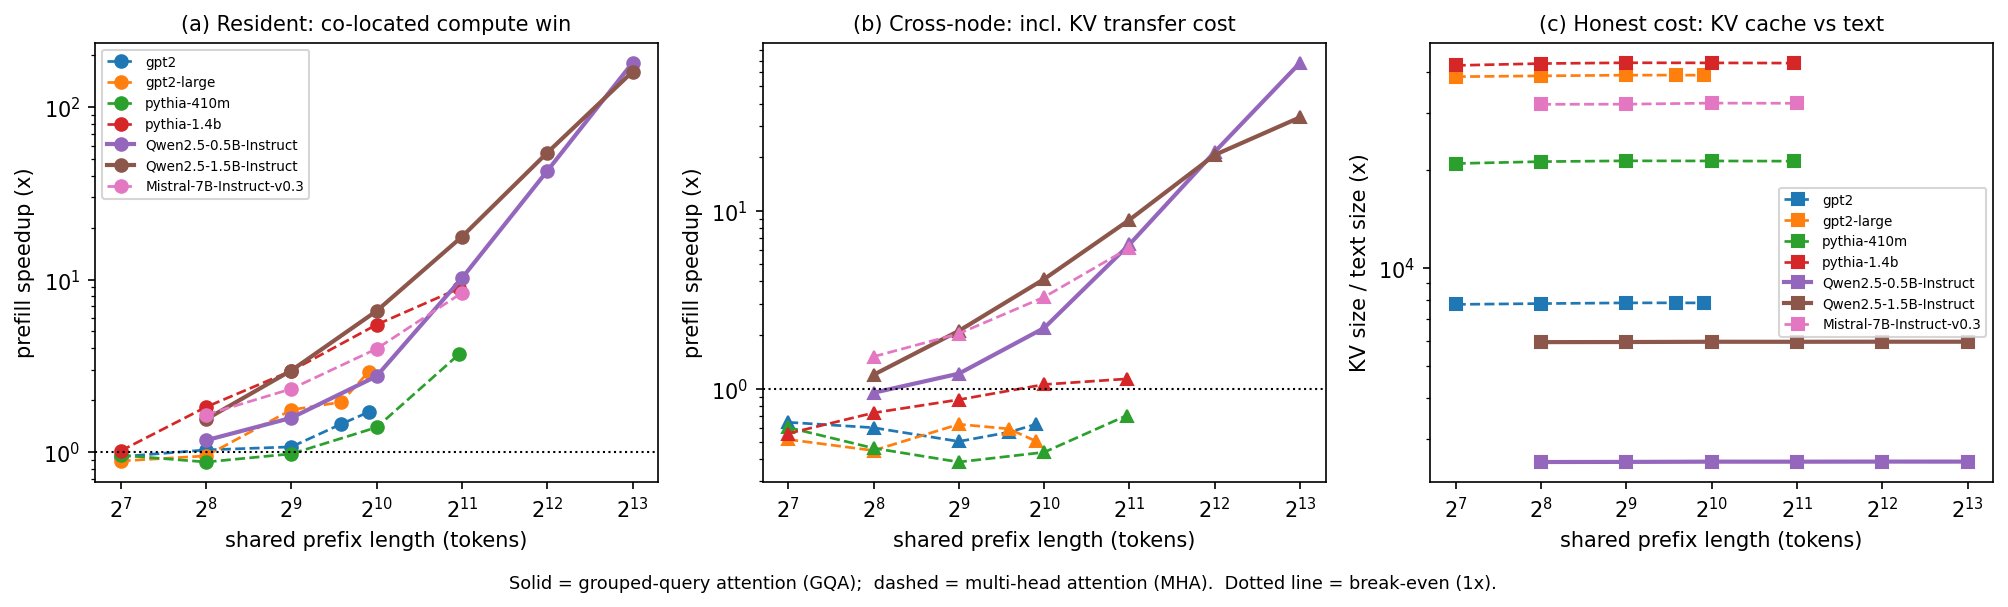
\includegraphics[width=\textwidth]{figures/fig_kv_bridge.png}
\caption{KV-bridge prefill reuse across seven models on an NVIDIA T4 (36 cells, log scales). (a)~Resident
speedup grows with prefix length and is dramatic for GQA models (solid), reaching $\sim$180$\times$ at
8k tokens. (b)~With KV transfer charged, GQA stays above break-even while MHA (dashed) mostly does not.
(c)~The KV cache is thousands of times larger than the text, and far larger for MHA than GQA --- the
reason transfer cost flips the verdict by architecture.}
\label{fig:kv}
\end{figure}

\begin{table}[t]\centering\footnotesize
\begin{tabular}{llrrrrl}
\toprule
Model & Attn & Max prefix & KV/text & Resident & Cross-node & Lossless \\
\midrule
GPT-2 (124M)      & MHA & 960  & 7.8k  & 1.7$\times$   & 0.6$\times$  & 4/5 \\
GPT-2-large (774M)& MHA & 960  & 39k   & 2.9$\times$   & 0.5$\times$  & 5/5 \\
Pythia-410M       & MHA & 2000 & 21k   & 3.7$\times$   & 0.7$\times$  & 5/5 \\
Pythia-1.4B       & MHA & 2000 & 43k   & 8.9$\times$   & 1.1$\times$  & 5/5 \\
Mistral-7B (4-bit)& MHA & 2048 & 32k   & 8.4$\times$   & 6.2$\times$  & 4/4 \\
Qwen2.5-0.5B      & GQA & 8192 & 2.5k  & \textbf{181$\times$} & \textbf{68$\times$} & 6/6 \\
Qwen2.5-1.5B      & GQA & 8192 & 5.9k  & \textbf{161$\times$} & \textbf{34$\times$} & 6/6 \\
\bottomrule
\end{tabular}
\caption{KV-bridge at each model's longest tested prefix. Resident = co-located compute win; cross-node
charges KV transfer. KV/text is the cache size relative to the text it replaces. Lossless counts cells
with byte-identical greedy output (35/36 overall).}
\label{tab:kv}
\end{table}

\noindent Three things come out of the run, and they match the hypothesis that motivated the gating
policy. First, reuse is a \emph{real} compute saving: once the shared prefix passes a crossover of a few
hundred tokens, the resident speedup climbs steeply --- to roughly $180\times$ for the half-billion-
parameter Qwen at an 8k prefix, because recompute pays $O(n^2)$ attention over the whole prefix while
the bridge pays only for the short query. Below the crossover the two are within noise ($\sim$0.9--1.1$\times$),
which is exactly why the policy does not bridge tiny contexts. Second, the saving is essentially
\emph{lossless}: 35 of 36 cells produced byte-identical greedy output. The single exception (GPT-2 at a
512-token prefix) is a one-token divergence from float16 rounding --- prefilling the whole sequence and
prefilling the query on top of a reused cache accumulate rounding slightly differently --- and would
disappear in float32; we report it rather than hide it. Third, and most decisive for the architecture,
the KV cache is \emph{thousands} of times larger than the text it stands in for (Table~\ref{tab:kv}),
and the ratio depends sharply on attention design: grouped-query models (Qwen, two KV heads) carry an
order of magnitude less cache than multi-head models (GPT-2-large, twenty heads). The consequence shows
up in the cross-node column: once the transfer cost of moving that cache is charged, GQA models stay
comfortably above break-even (Qwen reaches $68\times$) while most MHA models fall below it. In other
words, KV-bridge is worth it exactly when the producer and consumer are co-located \emph{or} the model
uses grouped-query attention --- which is precisely the condition \texttt{RegistryKvTransport} encodes,
falling back to \textsc{Ctx\_Ref} otherwise. The measurement grounds the policy rather than assuming it.

\section{Discussion and Limitations}\label{sec:disc}
Pulling the threads together: transcript accumulation is wasteful, and both summarizing and referencing
fix it without hurting accuracy on the tasks we tried. Summarizing is cheaper in tokens but throws
information away, which costs accuracy the moment a later step needs a discarded fact; referencing
costs a little more but keeps the information and carries provenance with it. KV transfer is a separate
lever again, paying off in compute when the shared prefix is long and the model is friendly to it. None
of these dominates, which is the whole point. We would also flag the retracted Haiku regression as a
result in its own right: it looked real at $n{=}1$ and evaporated at $n{=}5$, a reminder that a single
agent generation is not a measurement.

We would rather name the soft spots than have a reviewer find them. The biggest is breadth of models.
The token and losslessness experiments run on Claude Haiku, Sonnet, and Opus, which share a tokenizer
and an architecture family, so strictly speaking this is one family at three scales, not a cross-vendor
study, and the token counts in particular are tokenizer-specific. The KV-bridge experiment does span
seven open models and three attention designs, but that breadth lives on the compute side; the token
and accuracy story does not yet have it. Closing that gap is the single most valuable next run, and we
ship a notebook (\S\ref{sec:lossless}) that re-runs the losslessness test verbatim on an open model so
it is a button-press rather than a rewrite.

Sample size and scenario diversity are the next concern. The token comparison is one scenario with a
fixed upstream and only three samples per Sonnet/Opus cell, so those per-cell ratios are indicative
rather than tight. The losslessness experiment is a single pre-registered document; it cleanly shows
that a faithful summary drops facts and that a task needing one then fails, but it cannot tell us how
\emph{often} real workloads land in that situation. We are careful to claim existence, not frequency.
Establishing frequency would mean running the same protocol over several document types --- a contract
with exact obligations, a spec with exact thresholds, narrative text --- at larger $n$, and reporting
whichever way it comes out.

The security result is genuine but deliberately modest in what it proves. Forty injection attempts
across nine categories are all blocked with no false positives, and the chaining and obfuscation cases
are there to show that the decision ignores the text entirely. But that same property means the corpus
mostly confirms the lattice is implemented as specified; the interesting attacks live where the lattice
makes no promise, and we say so by including two boundary cases it does not stop --- an injection that
stays inside an allowed capability, and content mislabeled at ingress. A real security evaluation would
push on exactly those: the tagging boundary, a compromised broker, and output-side manipulation that a
capability gate cannot see.

Two scope notes finish the list. The KV-bridge numbers are microbenchmarks of a single prefill step on
one T4, measured against full recompute rather than against provider prefix-caching, which is the
comparison a deployment would actually care about and which we do not claim to beat; the ``transfer''
is a local serialize/deserialize rather than a network hop, and the one float16 divergence in
thirty-six cells means ``lossless'' here is token-identical in practice, not bit-exact in theory. And
the implementation is a single in-memory broker process. That matters for our third argument:
systematization only really shows up at scale, across many machines and restarts, and that is precisely
the setting we have not built. We therefore present systematization as a design goal rather than a
measured result, and treat a persistent, distributed store as future work, not as something this paper
has demonstrated.

\section{Future Work}\label{sec:future}
Three things would move this from a careful pilot to a result that travels. First, the cross-vendor
replication: run the token and losslessness experiments on at least one non-Claude model
(Llama-3.1-8B or Qwen2.5-7B are enough), since even a single open-model run removes the
single-family caveat that currently shadows half the paper. Second, breadth on the two thin
experiments: several document types for losslessness at $n\!\ge\!10$ each, and a security corpus that
attacks the parts the lattice does not guarantee --- ingress mislabeling and within-capability steering
--- rather than the part it does. Third, the engineering that the systematization claim is really
about: a durable, distributed context store (a persistent backing store with restart survival is the
honest first step), message signing and cross-reconnect replay nonces, and a head-to-head against
provider prefix-caching for the KV path. None of these change the design; they are about earning the
claims the design implies.

\noindent\textbf{On novelty.} We claim none for the mechanism --- shared stores, references, and KV
reuse all predate us. The contribution is the measured, reproducible accounting that ties them
together: a summarizer beats referencing on tokens, a summary's lossiness costs accuracy when a dropped
fact is needed, the capability lattice contains the attacks it was built for and openly not the ones it
was not, and KV transfer's compute win and storage cost are mapped across seven models --- with an
architecture that makes the byte/token split and the materialization choice explicit rather than
implicit.

\section{Conclusion}
Two measurements, on two cost planes, point the same way. On tokens, reference-minimization removes the
waste of transcript accumulation at no measured accuracy cost --- but it is not the cheapest option, a
competent summarizing orchestrator saves more, so TOAP earns referencing's place through losslessness,
in-band security, and systematization rather than raw token count. On compute, transferring a same-model
KV cache is a real, near-lossless prefill speedup that grows to two orders of magnitude on long contexts,
yet the cache is so much larger than the text that it only pays off co-located or under grouped-query
attention. The common thread is that no single way of sharing context dominates: the right choice
depends on length, architecture, co-location, and whether lossiness is acceptable --- which is the case
for making materialization an adaptive, cost-model-driven decision rather than a fixed mechanism. We
release all artifacts and call for cross-vendor, large-$n$, harder-task replication --- especially a
task that stresses the lossless-versus-lossy distinction, and a comparison of KV-bridge against provider
prefix-caching --- before any general claim.

\begin{thebibliography}{9}
\bibitem{erman1980} L.\ Erman, F.\ Hayes-Roth, V.\ Lesser, D.\ Reddy. The Hearsay-II Speech-Understanding
System (blackboard model). \emph{ACM Computing Surveys} 12(2), 1980.
\bibitem{mcp} Anthropic. Model Context Protocol specification, 2024--2026. \url{https://modelcontextprotocol.io}.
\bibitem{a2a} Google / Linux Foundation. Agent2Agent (A2A) Protocol v0.3, 2025--2026. \url{https://a2a-protocol.org}.
\bibitem{adol} Z.\ Chang, J.\ Li, Z.\ Cao. A Token-Efficient Data Layer for Agents (ADOL). IETF
Internet-Draft \texttt{draft-chang-agent-token-efficient-01}, Dec.\ 2025.
\bibitem{promptcache} Anthropic, OpenAI, Google. Prompt caching documentation, 2024--2026.
\bibitem{talkhier} Z.\ Wang et al. Talk Structurally, Act Hierarchically (TalkHier). arXiv:2502.11098, 2025.
\bibitem{codeagents} CodeAgents: pseudocode-codified multi-agent messages. arXiv:2507.03254, 2025.
\bibitem{camel} Google DeepMind. Defeating Prompt Injections by Design (CaMeL). arXiv:2503.18813, 2025.
\bibitem{kvcomm} KVCOMM: Online Cross-context KV-cache Communication. arXiv:2510.12872, 2025.
\end{thebibliography}

\appendix
\section{Reproducibility}
Artifacts: \texttt{benchmark/ab\_study/} (harness, scenarios, the $n{=}33$ run records
\texttt{runs/writer\_runs.json}, deterministic scorer \texttt{writer\_experiment.py}, analysis
\texttt{compute\_writer.py}); \texttt{paper/figures/} (figure scripts); \texttt{paper/METHODS.md} and
\texttt{paper/REVIEW\_RESPONSE.md} (method log and the reviewer-fix trail). The Rust implementation is
in \texttt{crates/} (29 unit + integration tests, incl.\ real-TCP end-to-end, V2 binary round-trip,
capability-lattice flow, cache layout, and KV-bridge fallback). Token reductions recompute exactly
from the committed records via \texttt{compute\_writer.py}.
\end{document}
